\section{Use cases identification}
\subsection{Scenarios}
Here are some scenarios that describe the usage of the system.
\subsubsection{Scenario 1}
\label{scenario:1}
Francesco wants to have a beer with his friend Vincenzo so Francesco logs in to system and searches for cars nearby. He notices that there are two cars available next to his house, he decides to reserve the one with more battery and after few minutes he reaches it. He starts to drive until he reaches Vincenzo's house, Vincenzo gets into the car and they arrive to the beer house where they terminate the rent.

\subsubsection{Scenario 2}
\label{scenario:2}
Mirjana has been told by her friend Elisa that a new car sharing service is available in their city and so she decided to give it a try as she wants to go shopping in the city center. She registers to the system providing all information requested, she inserts the destination address and enables the money saving option. She is provided by the system with a charging station not far from the shopping center and, as it is a sunny day, she decided to take that location as destination in order to achieve a discount and reach the shopping center on foot. 

\subsubsection{Scenario 3}
\label{scenario:3}
Giovanni is really interested in electric cars so he decides to use the PowerEnJoy system. He wants to go to the museum in the afternoon so he reserves a car. After one hour he is \todo{is he notified?}notified by the system that his reservation is expired and he is charged of a 1\euro\ fee. When he is ready to exit his house he notices that the same car is still available so he reserves it again, reaches it and starts driving. When he arrives at the destination he sees a charging station next to the museum so he decides to leave the car there plugging the charging cable in order to get a discount.

\newpage\subsection{Use case diagram}
\begin{figure}[h]
			\centering
			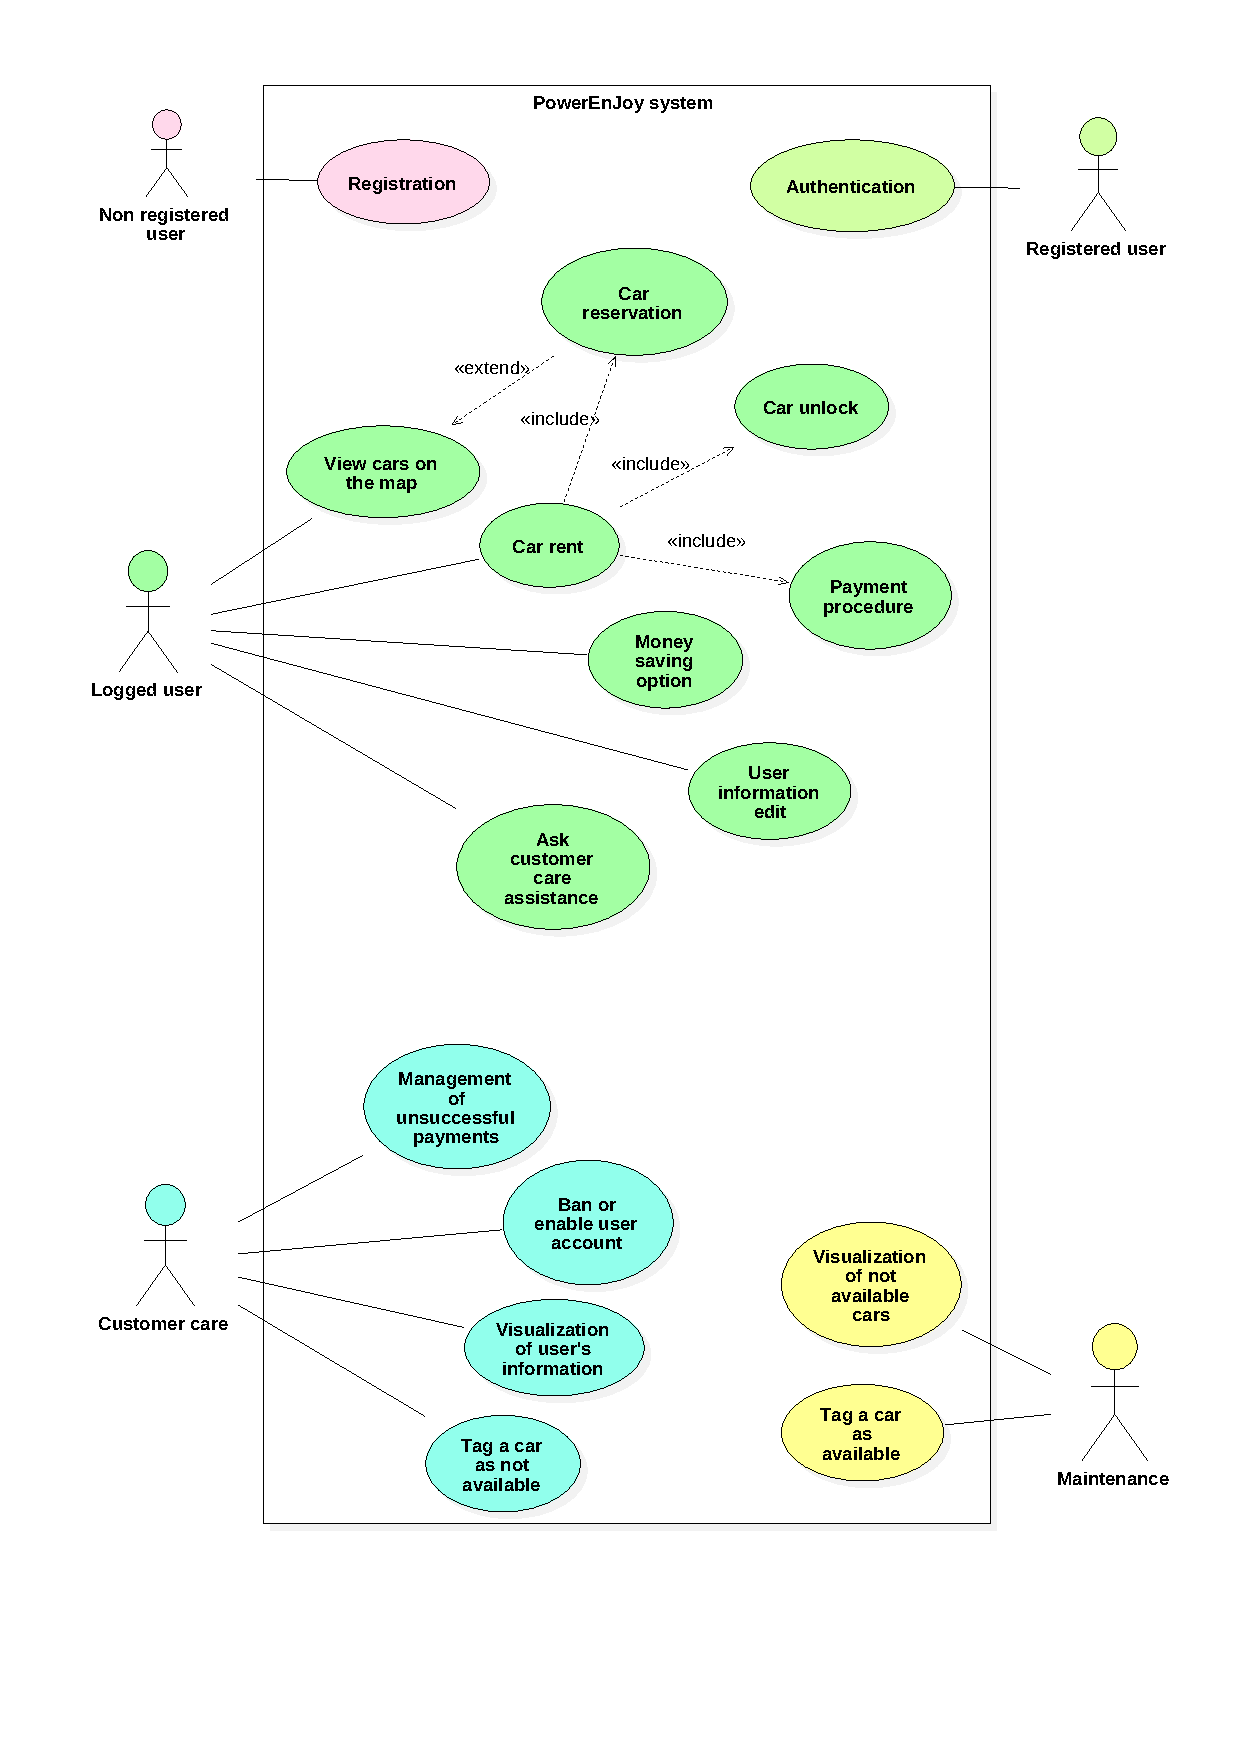
\includegraphics[width=0.9\textwidth]{useCase}
			\caption{
				\label{fig:useCase} 
				Use case diagram
			}
		\end{figure}
\subsection{Use cases description}
\begin{tabular}{p{0.25\linewidth}p{0.75\linewidth}}
\toprule
\textbf{Name} & \textbf{Authentication} \\
\midrule
\textbf{Actors} &  Registered user \\
\midrule
\textbf{Entry conditions} & The user must know his username and password \\
\midrule
\textbf{Flow of events} & 
\begin{enumerate}
	\item The user inserts his username and password in the appropriate form and submit it
	\item The system validates the inserted credential
	\item The system checks if the user is banned
\end{enumerate} \\
\midrule
\textbf{Exit conditions} & If the credential validation is successful the user is not banned he is granted the proper privileges\\
\midrule
\textbf{Exceptions} & 
\begin{itemize}
	\item If the credential validation failed an error message is displayed
	\item If the credential validation is successful and the user is banned a message providing assistance is displayed and the system doesn't allows the user to access to the system
\end{itemize} \\
\bottomrule
\end{tabular}

\begin{tabular}{p{0.25\linewidth}p{0.75\linewidth}}
\toprule
\textbf{Name} & \textbf{Car reservation} \\
\midrule
\textbf{Actors} &  Registered user \\
\midrule
\textbf{Entry conditions} & The user must be logged in \\
\midrule
\textbf{Flow of events} & 
\begin{enumerate}
	\item The user chooses if he wants to use his GPS position or insert a different one manually
		\subitem a. The system retrieves the user's  GPS position
		\subitem b. The user inserts a position
	\item The system retrieves the position of all available cars
	\item The system shows a map with all available cars near the position indicated by the user
	\item The user selects a car he wants to reserve
	\item The system show the user informations about car battery percentage
	\item The user confirms he wants to reserve that car
\end{enumerate} \\
\midrule
\textbf{Exit conditions} & The system set the state of the car as \emph{Reserved} paired with the user who made the reservation\\
\midrule
\textbf{Exceptions} & 
If the position inserted by the user is not correct an error message is displayed \\
\bottomrule
\end{tabular}

\begin{tabular}{p{0.25\linewidth}p{0.75\linewidth}}
\toprule
\textbf{Name} & \textbf{Car unlock} \\
\midrule
\textbf{Actors} &  Registered user \\
\midrule
\textbf{Entry conditions} & 
\begin{itemize}
	\item The user must be logged in
	\item The user should have done a reservation for a car
\end{itemize} \\
\midrule
\textbf{Flow of events} & 
\begin{enumerate}
	\item The user select the unlock button to ask the system to unlock the car
	\item The system checks if the user credentials corresponds to the credential of the user paired with the \emph{Reserved} state of the car
	\item The system checks if the user's position is at most 5 meters away from the position the car he reserved
	\item The system unlocks the car
\end{enumerate} \\
\midrule
\textbf{Exit conditions} & The car is unlocked and the user may enter it\\
\midrule
\textbf{Exceptions} & 
\begin{itemize}
	\item If the user credentials doesn't correspond to the credential of the user paired with the \emph{Reserved} state of the car the system displays an error message
	\item If the position of the user is not at most 5 meters away from the position the car he reserved the system displays an error message
\end{itemize} \\
\bottomrule
\end{tabular}

\begin{tabular}{p{0.25\linewidth}p{0.75\linewidth}}
\toprule
\textbf{Name} & \textbf{Car Rent} \\
\midrule
\textbf{Actors} &  Registered user \\
\midrule
\textbf{Entry conditions} & 
\begin{itemize}
	\item The user must be logged in
\end{itemize} \\
\midrule
\textbf{Flow of events} & 
\begin{enumerate}
	\item \emph{Car reservation}
	\item \emph{Car unlock}
	\item The user ignites the car enigne
	\item The system must set the state of the \emph{Reserved} car to \emph{In Use} paired
	with the same user
	\item During the rent the user is informed about the current charge and if it is or not inside a
	safe aerea
	\item The user leaves the auto turning off the engine
	\item The system locks the car
    \item The system activates a timer to allow the user to plug the car into a power grid if it is
    near one of them
	\item When the timer expires: \emph{Payment procedure}
	\item The system sets the car as \emph{Available}
\end{enumerate} \\
\midrule
\textbf{Exit conditions} & 
The user is charged of the correct amount for the ride and at anytime could perform another rent, the car is avaible again\\
\midrule
\textbf{Exceptions} & 
\begin{itemize}
	\item If the user doesn't unlocks the car up to one hour after the reservation, it is charged of 1\euro\, the car state is set as \emph{Available} and the user is notified by email his reservation is expired
	\item ...
\end{itemize} \\
\bottomrule
\end{tabular}

\begin{tabular}{p{0.25\linewidth}p{0.75\linewidth}}
\toprule
\textbf{Name} & \textbf{Payment procedure} \\
\midrule
\textbf{Actors} &  Registered user\\
\midrule
\textbf{Entry conditions} & 
\begin{itemize}
	\item The user must be logged in
	\item The user must have completed a rent
\end{itemize} \\
\midrule
\textbf{Flow of events} & 
\begin{enumerate}
	\item The timer activated by the system locking the car expires
	\item The system checks if the car position is or not inside a safe area
	\item The system checks if the car has detected more then one passenger during the rent
	\item The system checks the car battery percentage
	\item The system checks if the car is plugged on a charging station
	\item The system checks the distance of the car from the nearest charging station
	\item The system calculates the cost of the ride based on the rent time
	\item The system determines the applicable discounts/extra fee applying it to the cost of the ride
	\item The system starts a payment procedure with user's payment information using
	an external service
	\item The system logs data about the rent and the payment
	\item The system waits a response from the external payment service
    \item The system notifies through email the user about the result of the payment procedure and on discount/extra fees applied
\end{enumerate} \\
\midrule
\textbf{Exit conditions} & 
The user is charged of the correct amount for the ride\\
\midrule
\textbf{Exceptions} & 
\begin{itemize}
	\item If the payment procedure is not correctly completed, the user is banned, the payment suspended and the user is informed through mail to contact the customer service
	\item ...
\end{itemize} \\
\bottomrule
\end{tabular}